%!TEX root = ../Thesis.tex
\chapter{Introduction}
\label{sec:intro}

%--------------------------------------------------------------------------------
\clearpage
\section{Energy generation from the wind}
\label{sec:intro_engen}


%--------------------------------------------------------------------------------
\subsection{Motivation and global status}
\label{sec:intro_history}

Global energy systems are currently undergoing a revolution. The production of electricity for household and industrial use has, until the recent past, relied almost entirely on non-renewable fuel sources including coal and petroleum derivatives which are burned to run steam turbine generators. A number of compelling motives exist which are precipitating change to the status quo.

The first motivation being the overwhelming scientific evidence of the impacts of large scale releases of air pollutants into the environment. Particulates have been closely linked to lung (\cite{hamra_outdoor_2014}) and heart disorders (\cite{du_air_2016}). Carbon dioxide, a greenhouse gas, is also released through the combustion process and acts to increase the Earth's surface temperature through radiative forcing (\cite{charlson_climate_1992}), as well as acidify water bodies through the formation of carbonic acid and harming marine life (\cite{doney_ocean_2009}). Other pollutants including sulfur oxides and nitrogen oxides contribute to smog and acid rain, and are similarly linked to acute heath effects (\cite{brunekreef_air_2002}).

Realizing the urgency of these environmental concerns, authorities across the world have begun to enact agreements to curb their emissions contributions. These pacts can range from city and regional planning regulations, to national legislation and international treaties. Examples include the United Nations Kyoto Protocol and Paris Climate Agreement, European Commission's Clean Energy for all Europeans Framework (\cite{ec_clean_energy}), China's Renewable Portfolio Standard (\cite{china_rps}) and Denmark's Energy Strategy (\cite{danmark_energi}). In conjunction with improvements in energy efficiency, large impacts can be made by the exchange and supplementation of low-carbon, renewable based generation including wind and solar.

Beyond commitments to avoiding the negatives associated with hydrocarbon based fuels, new opportunities have emerged with the maturation specifically of the wind energy industry. Rapid cost decreases have been demonstrated through experience, competition, and scaling which have brought the levelized-cost-of-energy (LCOE) of onshore wind power within reach and in many areas below that of traditional power plants without the need for subsidies. The IRENA renewable cost database reveals a 2017 average global LCOE for onshore wind at 60 and offshore wind at 140 USD/MWh, with projections for further decreases in the coming years (\cite{IRENA_2018}). The 2019 tender for Saudi Arabia's first installation, the 400 MW Dumat Al Jandal wind farm, resulted in a record power purchase agreement (PPA) of 21.3 USD/MWh (\cite{masdar_edf_2019}).

A final rationale for embracing renewable energy development in many areas is the opportunity for leveraging locally available resources instead of relying on imported fuels from territories which are often rife with geopolitical conflicts. Ensuring security of supply for the local population through greater self-sufficiency can lead to more a balanced hegemony in regional and global politics.

While wind power only supplies about 4\% of global electricity demand at present (14\% in the European Union and 44\% in Denmark), the aforementioned developments have resulted in a large and rapid expansion of planned and installed projects worldwide. Figure \ref{fig:wind_power_cum} presents a timeline of cumulative globally installed wind power, with the 2017 aggregate totalling over 539 GW. The growth rate is projected to remain near 10\%, year on year (\cite{gwec_global_2017}) with many large projects already approved and financed for construction in the coming years.

\begin{figure}[htbp]
    \centering
        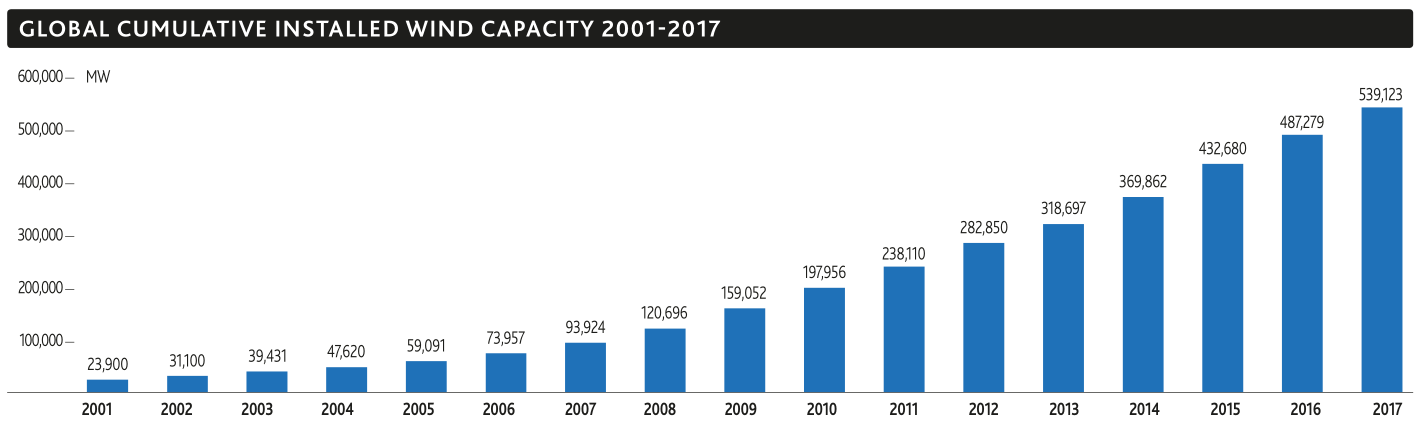
\includegraphics[width=1.0\textwidth]{graphics/intro/motivation_market/wind_power_cum.png}
    \caption{Cumulative worldwide installed wind power capacity from 2001-2017. The current value exceeding 539 GW. Source: \cite{gwec_global_2017}}
    \label{fig:wind_power_cum}
\end{figure}

%--------------------------------------------------------------------------------
\clearpage
\subsection{Intermittency of wind resource}
\label{sec:intro_intermittency}

The reliable and efficient exploitation of wind power faces a unique set of challenges. Electrical energy produced by wind turbines is derived from the kinetic energy of the wind. Air flow generates a lift force on the blades causing them to rotate. This mechanical energy ultimately drives the generator, producing electricity which is collected and fed to the power grid. As the wind is not a controllable fuel source, the turbine's output will to a large extent be determined by atmospheric conditions.

Winds originate from differential heating of the Earth's surface and are transported by bulk motion. Within the boundary layer, they are largely influenced by the planet's surface (terrain and vegetation), human made obstacles, weather systems, and turbulent mixing. 
%The wind consists of a mean dominant force in addition to irregular fluctuations (turbulence).
%varying levels of turbulence 
%turbulent kinetic energy (TKE) driven by atmospheric stability
% other interactions such as with thermal convective up/downdrafts and turbulent eddies

Wind variability is defined as the fluctuations in energy content of the wind. These variations occur across a wide range of temporal and spatial scales. Contributions can include diurnal, seasonal, and interannual patterns, and physical processes including: gravity waves, cold fronts, storms, cellular convection, convective rolls, low level jets, and sea breezes (\cite{vincent_forecasting_2017}). Combinations of these synoptic-, meso- and micro-scale influences lead to a high degree of intermittency in the wind, as shown in Figure \ref{fig:wind_speed_power_ts} using measurements shown with a sampling rate of 1-second.

\begin{figure}[htbp]
    \centering
        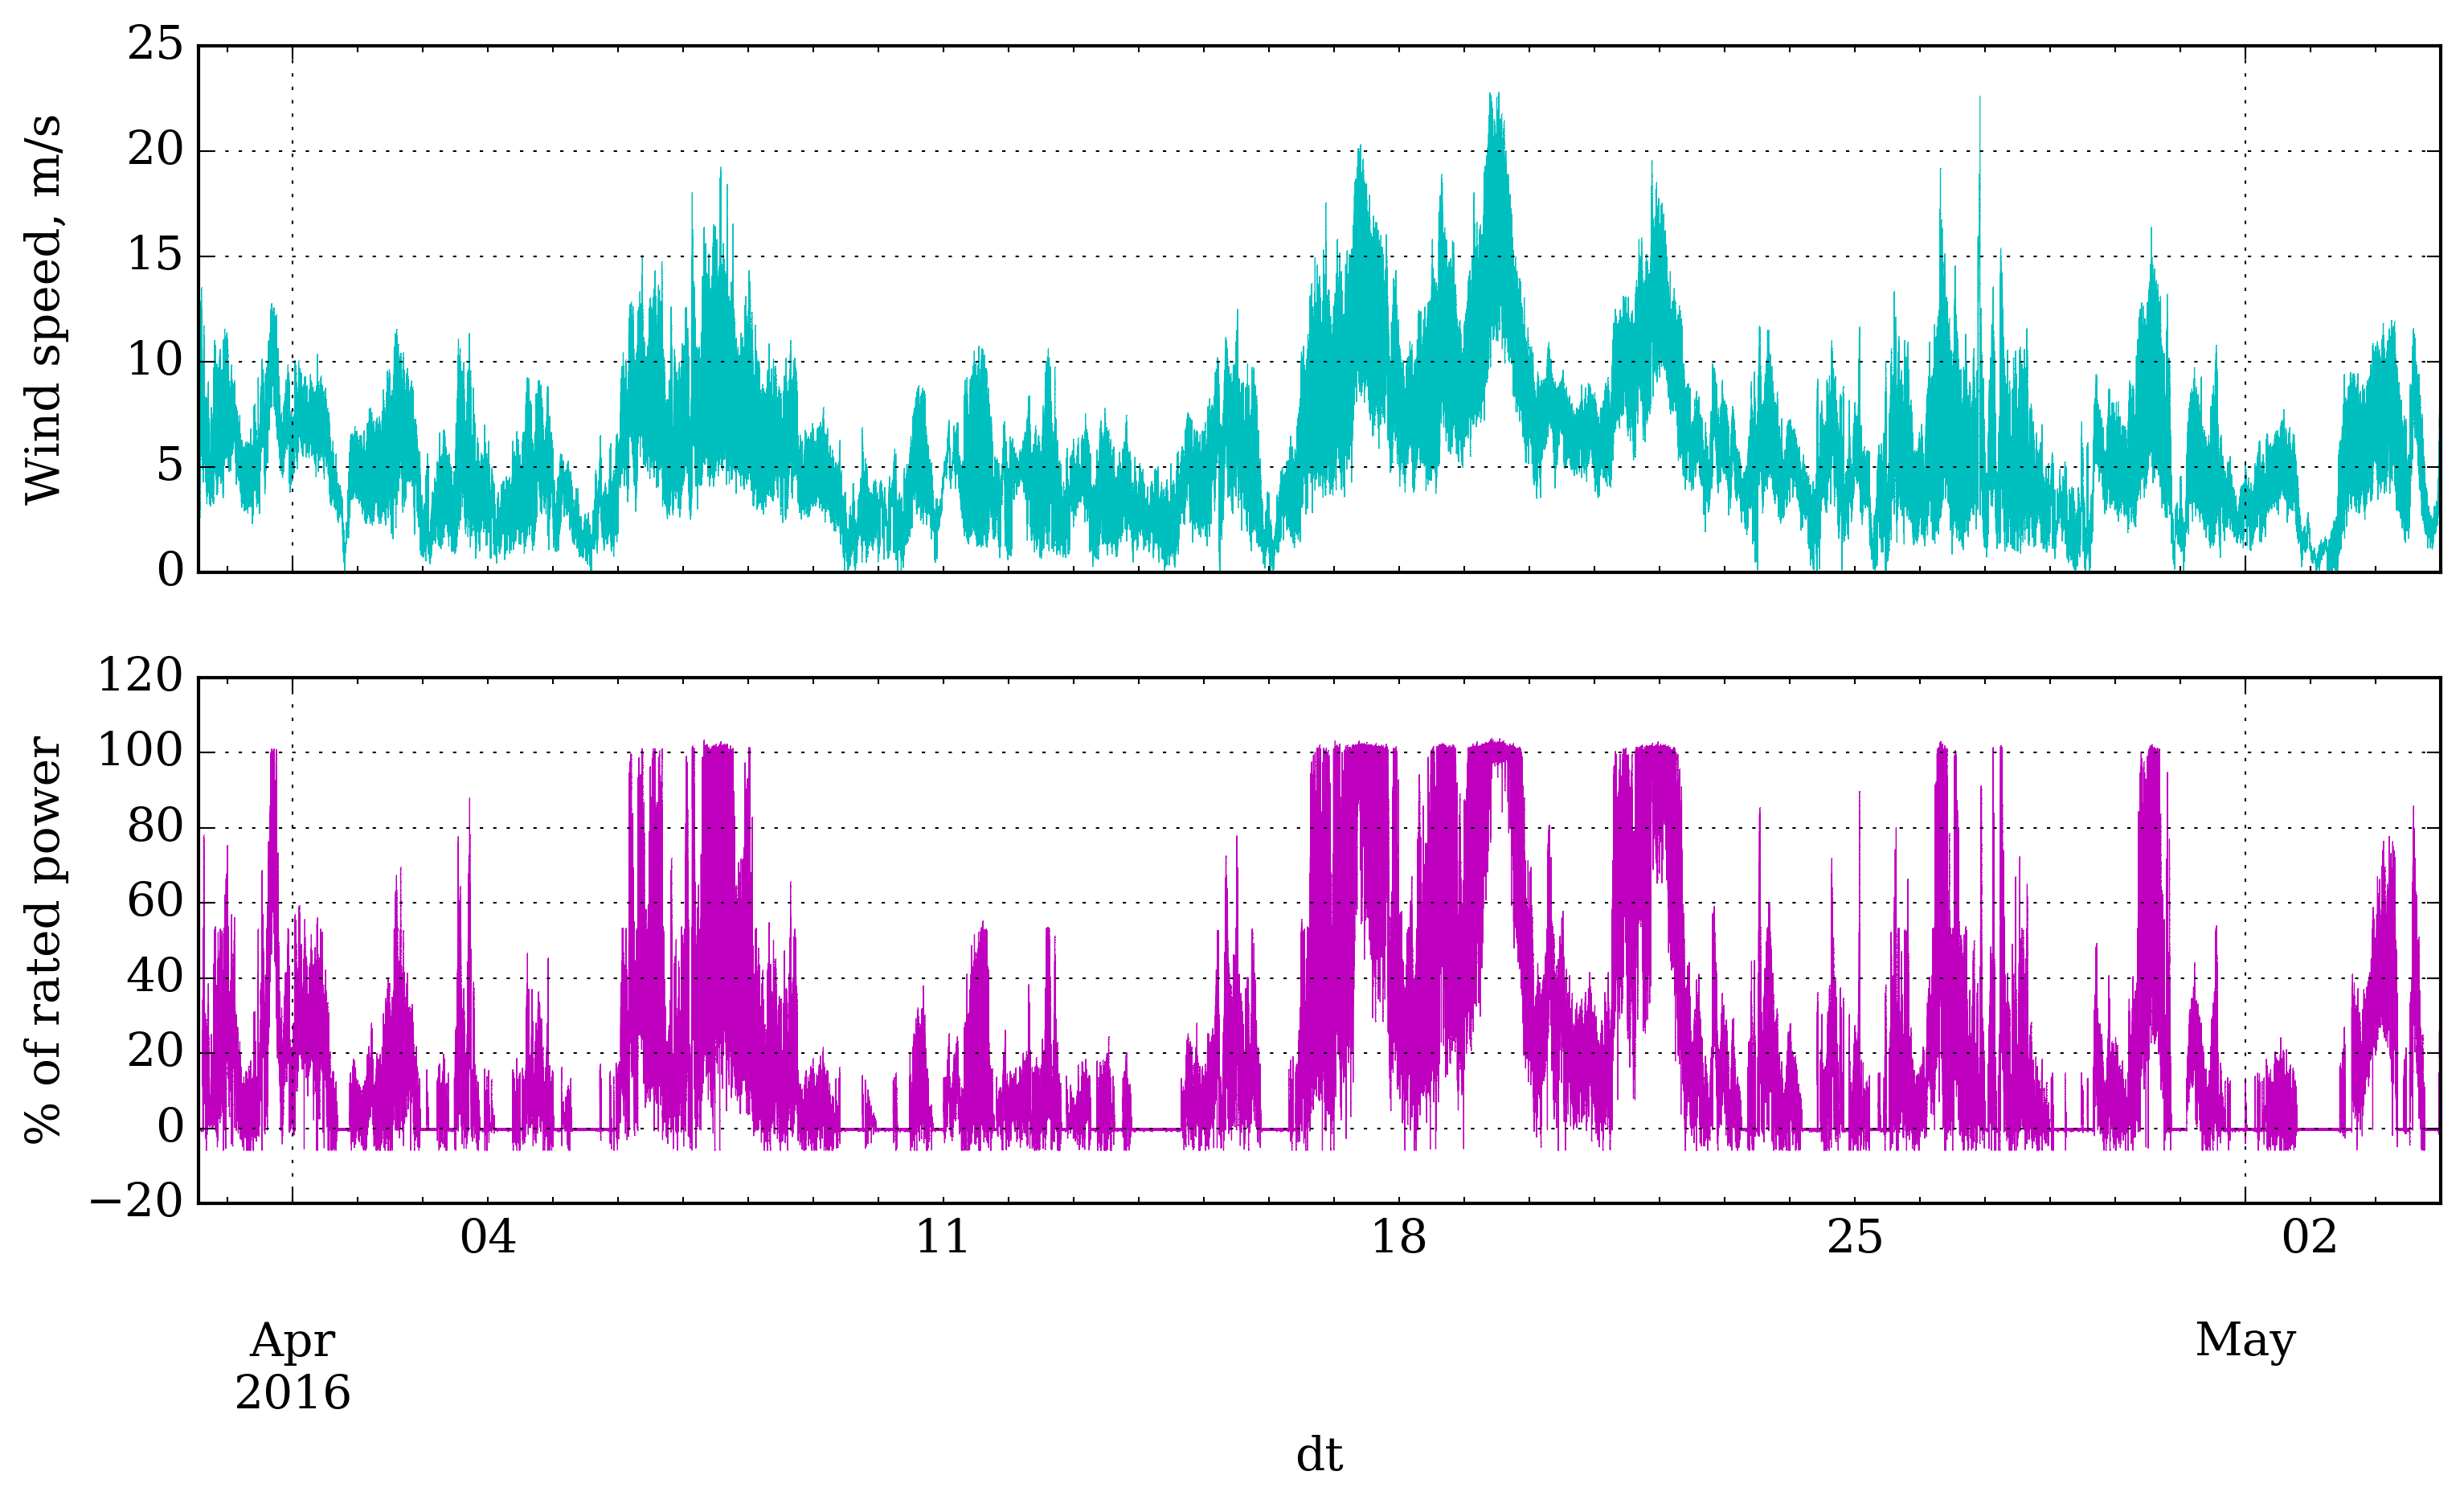
\includegraphics[width=1.0\textwidth]{graphics/intro/variability/wind_speed_power_ts.png}
    \caption{Time series example of wind speed (top) and wind power (bottom) variability from DTU's V52 research turbine}
    \label{fig:wind_speed_power_ts}
\end{figure}

Because the amount of extractable power from the wind is proportional to the cube of the wind velocity, relatively small differences in wind conditions can result in large deviations in power output. Wind ramps, or large and sudden changes in a turbine or wind farm's output are notoriously difficult to forecast (both the scale and timing) and can cause (in the best case) energy to be wasted (through curtailment during up-ramps), or in the worst case system-level shortages (during down-ramps). To prevent these possible shortages during periods of expected variability, reserve wind power can be secured through down-regulation (curtailment) which is then available for activation through flexible dispatch mechanisms.

Power spectral density (PSD) plots illustrate the distribution of energies which contribute to the signal's variability, ordered by frequency. An example is shown in Figure \ref{fig:wind_speed_power_psd} for wind speed and active power from a wind turbine using the same high-frequency dataset. This was obtained using Welch's method (\cite{welch_use_1967}) with Hamming windowing to reduce noise in the spectra. The trends indicate that the variability decreases with decreasing time-scales in both cases.

\begin{figure}[htbp]
    \centering
        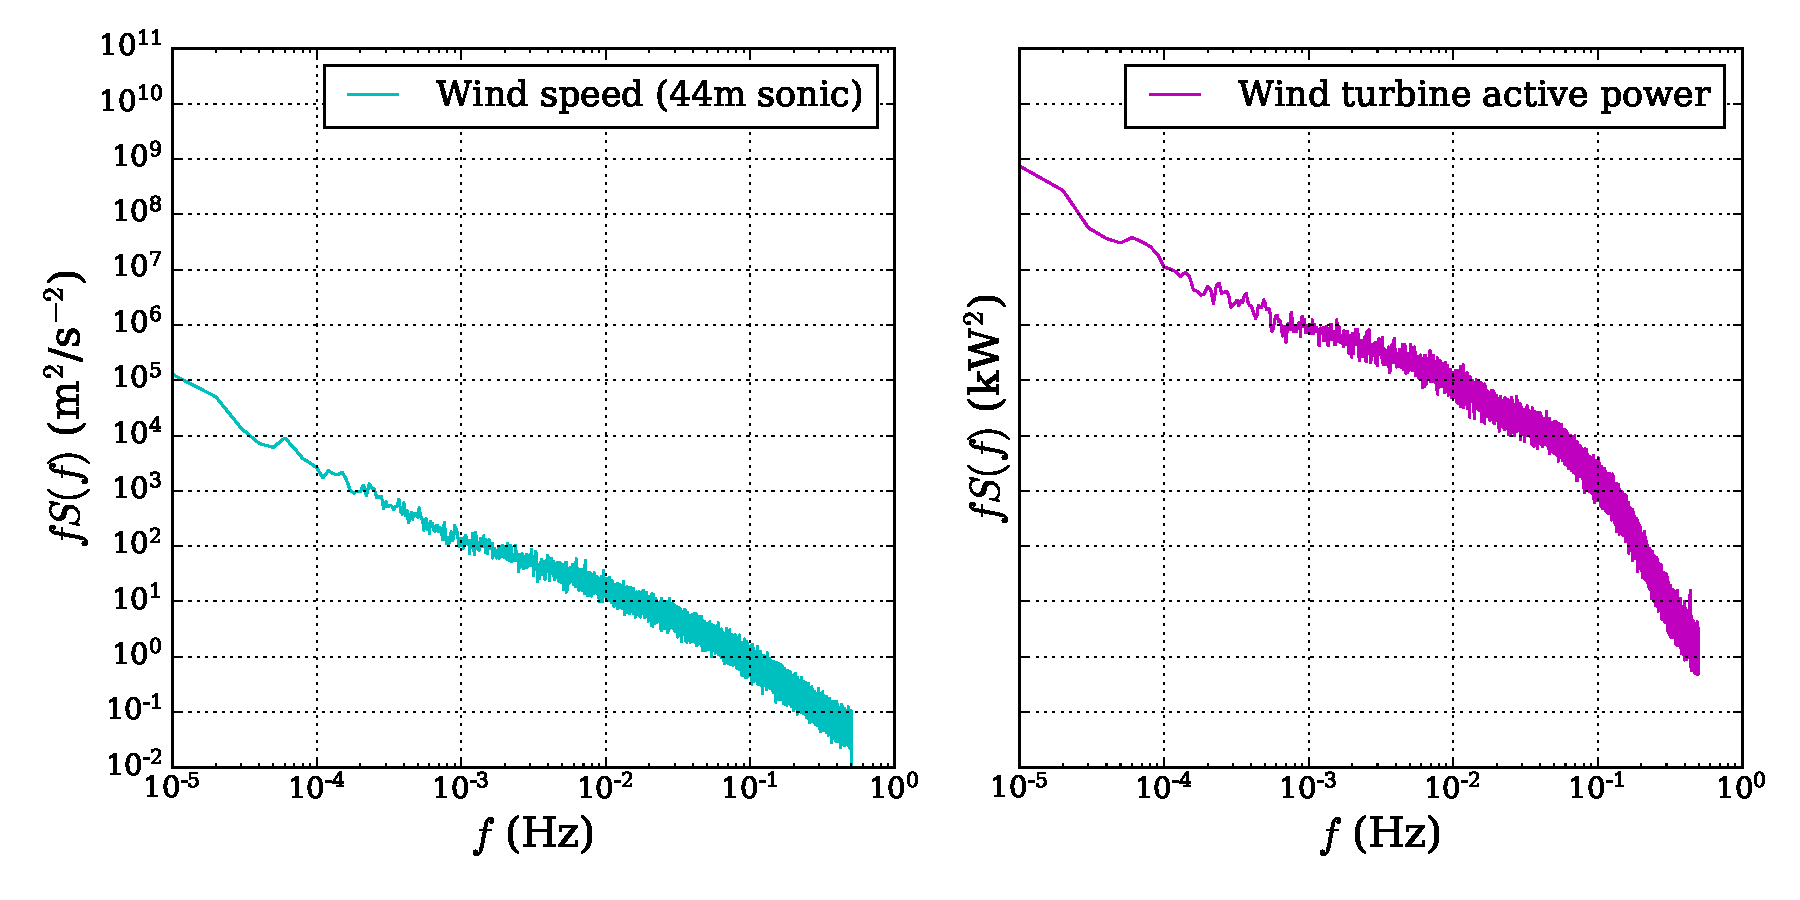
\includegraphics[width=1.0\textwidth]{graphics/intro/variability/wind_speed_power_psd.pdf}
    \caption{Power spectral density (PSD) of wind speed (left) and wind power (right) from DTU's V52 research turbine}
    \label{fig:wind_speed_power_psd}
\end{figure}

Without system level storage, wind power variability is mostly addressed by spatial smoothing. Averaging occurs firstly on the turbine level, where the fastest (millisecond-second scale) fluctuations are to a large extent compensated for by the inertia and swept area averaging of the wind turbine's rotor. Although individual turbine outputs within a wind farm are strongly correlated, their collective power output is smoothed on the second-minute scale by the aggregation effect. Most substantially, entire wind farms dispersed over large areas provide the largest impact towards reducing variability across all time scales due the low correlation of production between sites operating across different weather and geographic contexts. 

An in-depth report on integrating large shares of wind generation into power systems is available in \cite{holttinen_IEA25}, which provides further background and context for wind power variability in addition to relevant statistics and case studies.

\begin{comment}
The variability decreases as geographic area increases
Variability higher offshore

\cite{larsen_full_scale_2016} 
Wind motion exists Global atmospheric circulation originates from differential heating of the Earth's poles and equator which is rotated by the Coriolis force due to the planet's spin. Large scale circulation cells 
scales, turbulence etc.
large number of turbines are usually installed within a small geographical area, leading to correlated fluctuations between many turbines
    
balancing in high penetration
there are ideas for storage but none implemented at large scale at this time
real time balancing
\end{comment}

%--------------------------------------------------------------------------------
\clearpage
\subsubsection{Case study of wind turbine power variability}
\label{sec:intro_intermittency_V52}

To further explore wind variability and its impact on power systems, a summary investigation was conducted to characterize changes in electrical power output from a real world wind turbine. The data consists of high-resolution SCADA measurements from DTU's Vestas V52 research turbine at Ris{\o} (\cite{dtu_v52}). This model is one of the most commonly sold turbines worldwide and has a rated capacity of 850 kW. The sourced data spans from March 30 to May 4th, 2016 (35 days) during a calibration period when the turbine's control systems were under normal operation and no aerodynamic modifications were present. 

Measurements of the turbine's active power signal were down-sampled from 35 Hz to 1-second averages, and normalized with respect to rated power (where a value of 100 represents the generator's nameplate capacity). Note that it is possible to have both values below zero (during start up when drawing power from the grid) as well as values above 100 on the short term.

Statistics of absolute changes in the turbine's normalized power output within various time frames ranging from 1-second to 1-hour are presented in the following. Figure \ref{fig:act_pow_change_vioboxplot} presents a combined violin and boxplot across the selected time windows which illustrates statistical properties such as the shape and width of the distributions, quartile positions, median values, and spread of outliers. This is joined with Table \ref{tab:intro_v52_variability_statistics} describing summary statistics.

\begin{figure}[htbp]
    \centering
        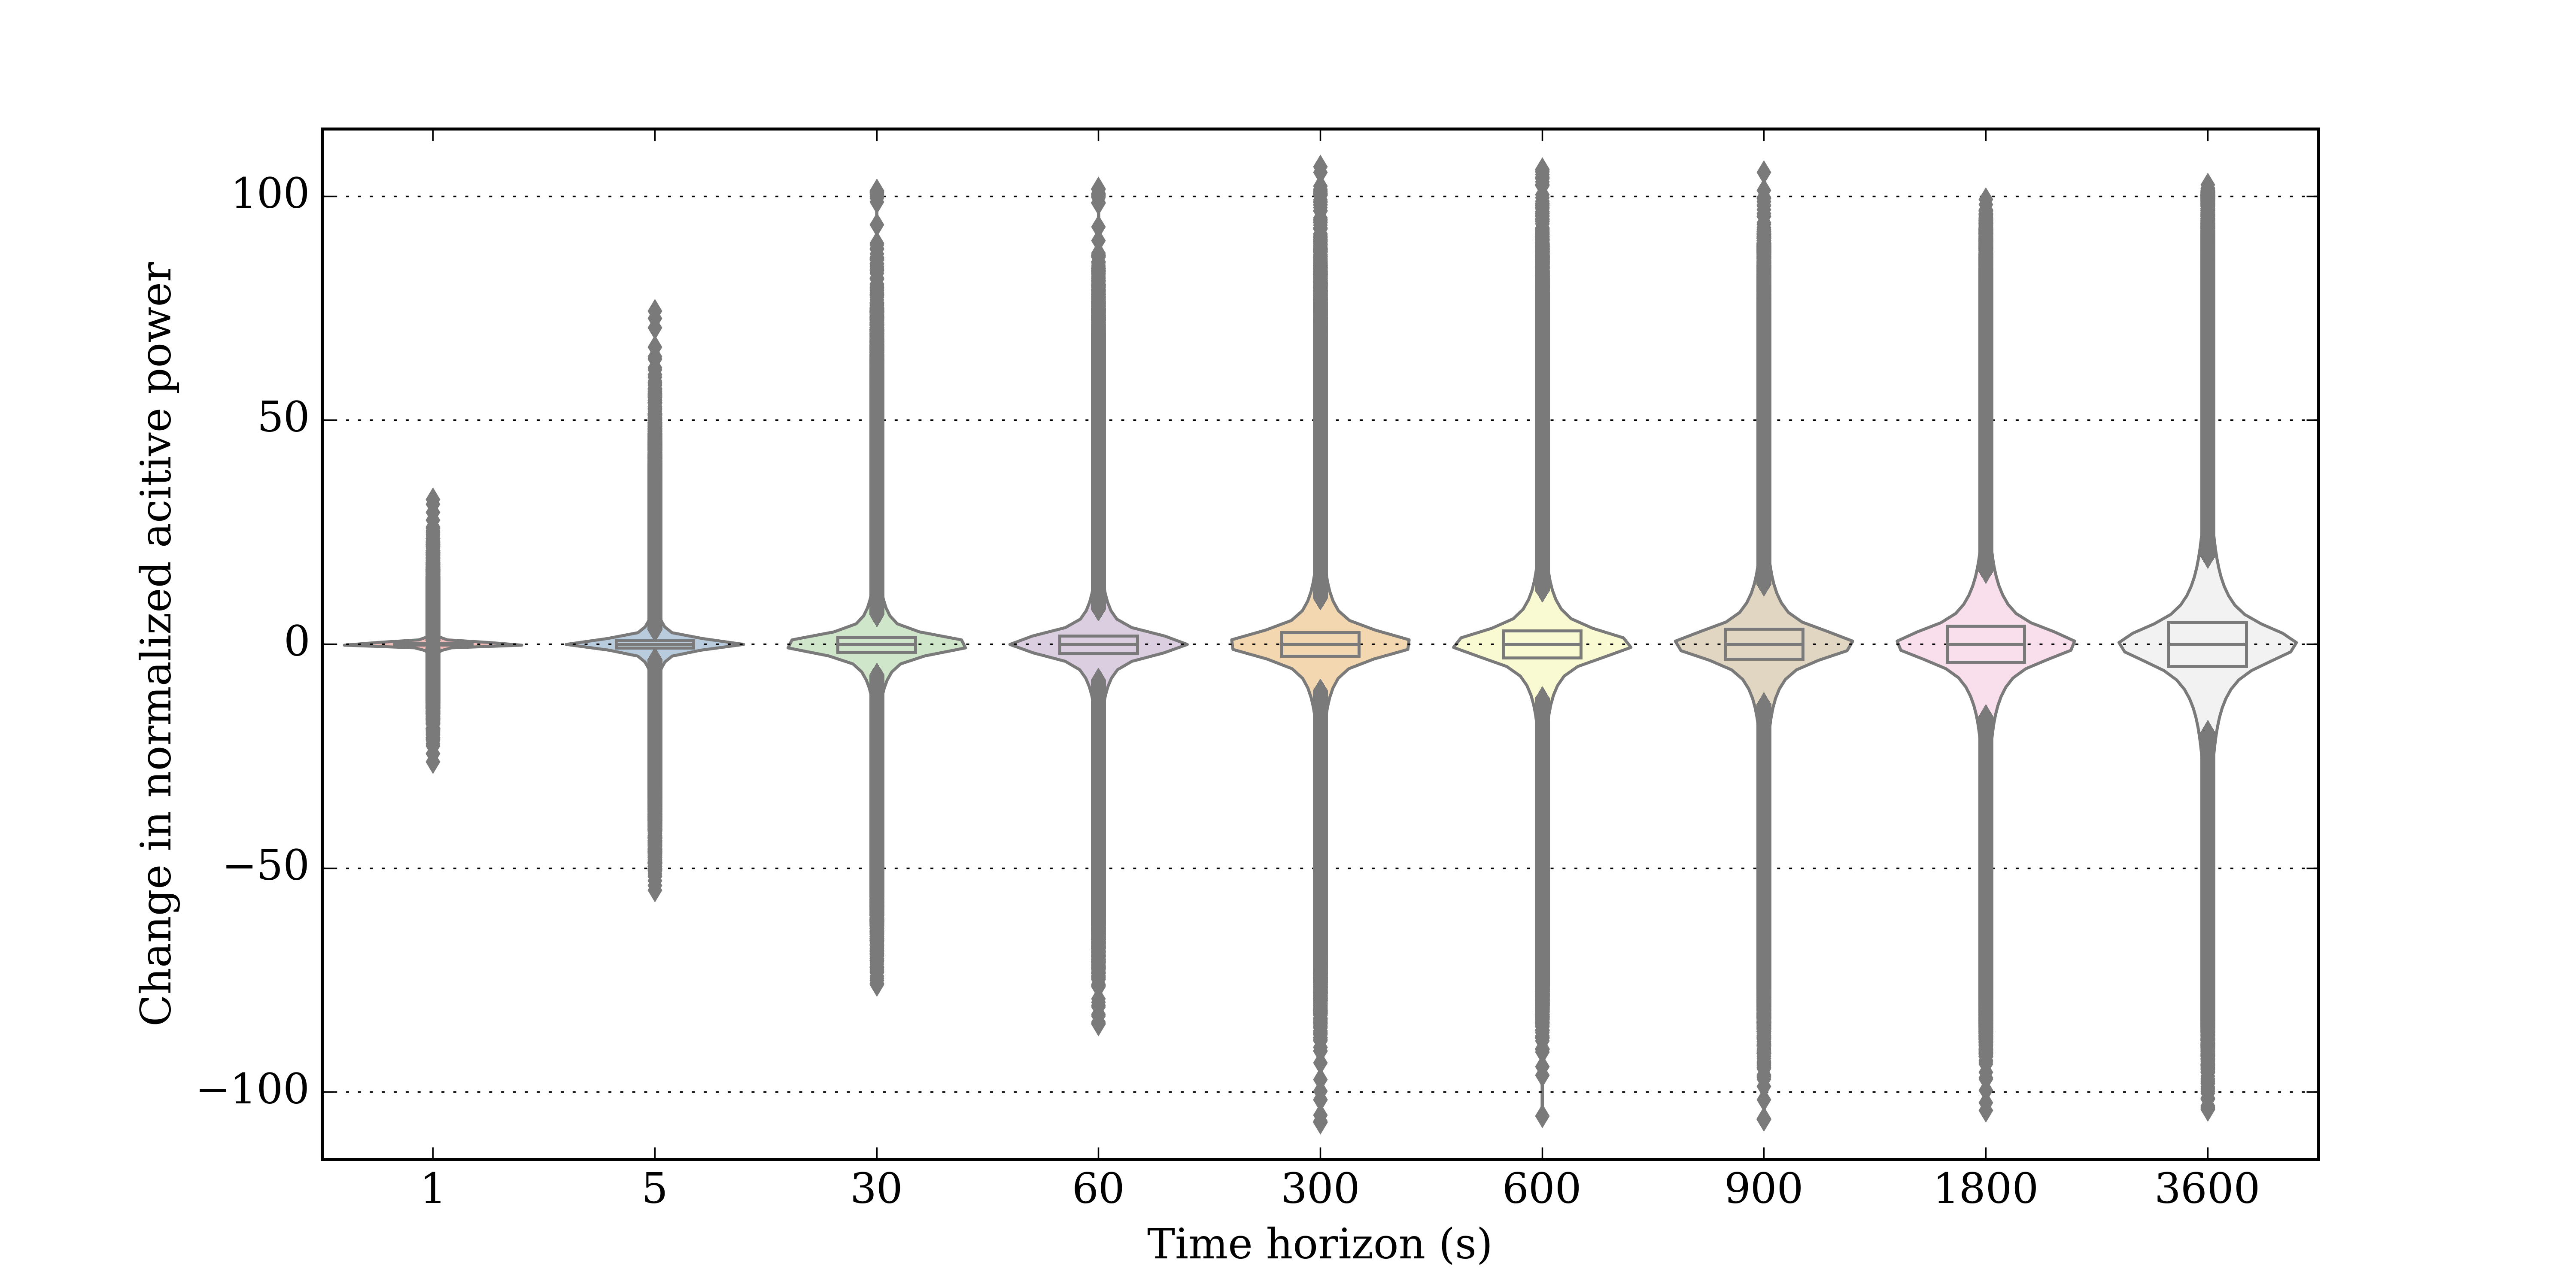
\includegraphics[width=1.0\textwidth]{graphics/intro/variability/act_pow_change_vioboxplot.png}
    \caption{Combined violin and boxplot of normalized active power changes by various time windows from DTU's V52 research wind turbine}
    \label{fig:act_pow_change_vioboxplot}
\end{figure}

\begin{table}
    \centering
    \caption{Table of statistics for V52 power output variability over selected time windows up to 1-hour}
    \resizebox{\columnwidth}{!}{%
\begin{tabular}{lrrrrrrrrr}
\toprule
{} &          1 s &          5 s &         30 s &         60 s &        300 s &        600 s &        900 s &       1800 s &       3600 s \\
\midrule
count &  2976599 &  2976595 &  2976570 &  2976540 &  2976300 &  2976000 &  2975700 &  2974800 &  2973000 \\
mean  &        0.000 &        0.000 &        0.000 &        0.000 &        0.002 &        0.003 &        0.004 &        0.008 &        0.009 \\
std   &        1.209 &        4.387 &        8.133 &        9.536 &       11.362 &       11.976 &       12.532 &       13.674 &       15.485 \\
min   &      -26.250 &      -54.907 &      -76.028 &      -84.816 &     -106.745 &     -105.303 &     -106.126 &     -104.044 &     -103.887 \\
25\%   &       -0.225 &       -0.888 &       -1.841 &       -2.103 &       -2.630 &       -3.075 &       -3.371 &       -4.049 &       -4.957 \\
50\%   &        0.000 &        0.000 &        0.000 &        0.000 &        0.000 &        0.000 &        0.000 &        0.000 &        0.000 \\
75\%   &        0.214 &        0.782 &        1.515 &        1.860 &        2.544 &        2.972 &        3.341 &        4.064 &        4.870 \\
max   &       32.326 &       74.414 &      101.242 &      101.663 &      106.567 &      106.013 &      105.350 &       99.266 &      102.539 \\
\bottomrule
\end{tabular}
}
    \label{tab:intro_v52_variability_statistics}
\end{table}

As expected, the variability grows with the length of the window. In all cases, the mean and median power output change is very close to zero and probability densities are symmetrical (normally distributed). On the very shortest timescales (1 and 5-seconds), the variations within the interquartile range (IQR) are small. However, from 30-seconds to 1-minute windows, the spread grows considerably. By the 5-minute case (300 s), the standard deviation approaches that of the longer timescales.

This is further shown in Figure \ref{fig:norm_act_pow_error_dist}, where the distributions are stacked atop each other for comparison (note the logarithmic y-axis scaling). Tail bumps present for certain time windows near the peripheries indicate periods of automatic start up (right tail) when the cut-in wind speed is reached and shut down (left tail) when the cut-out wind speed is exceeded.

\begin{figure}[htbp]
    \centering
        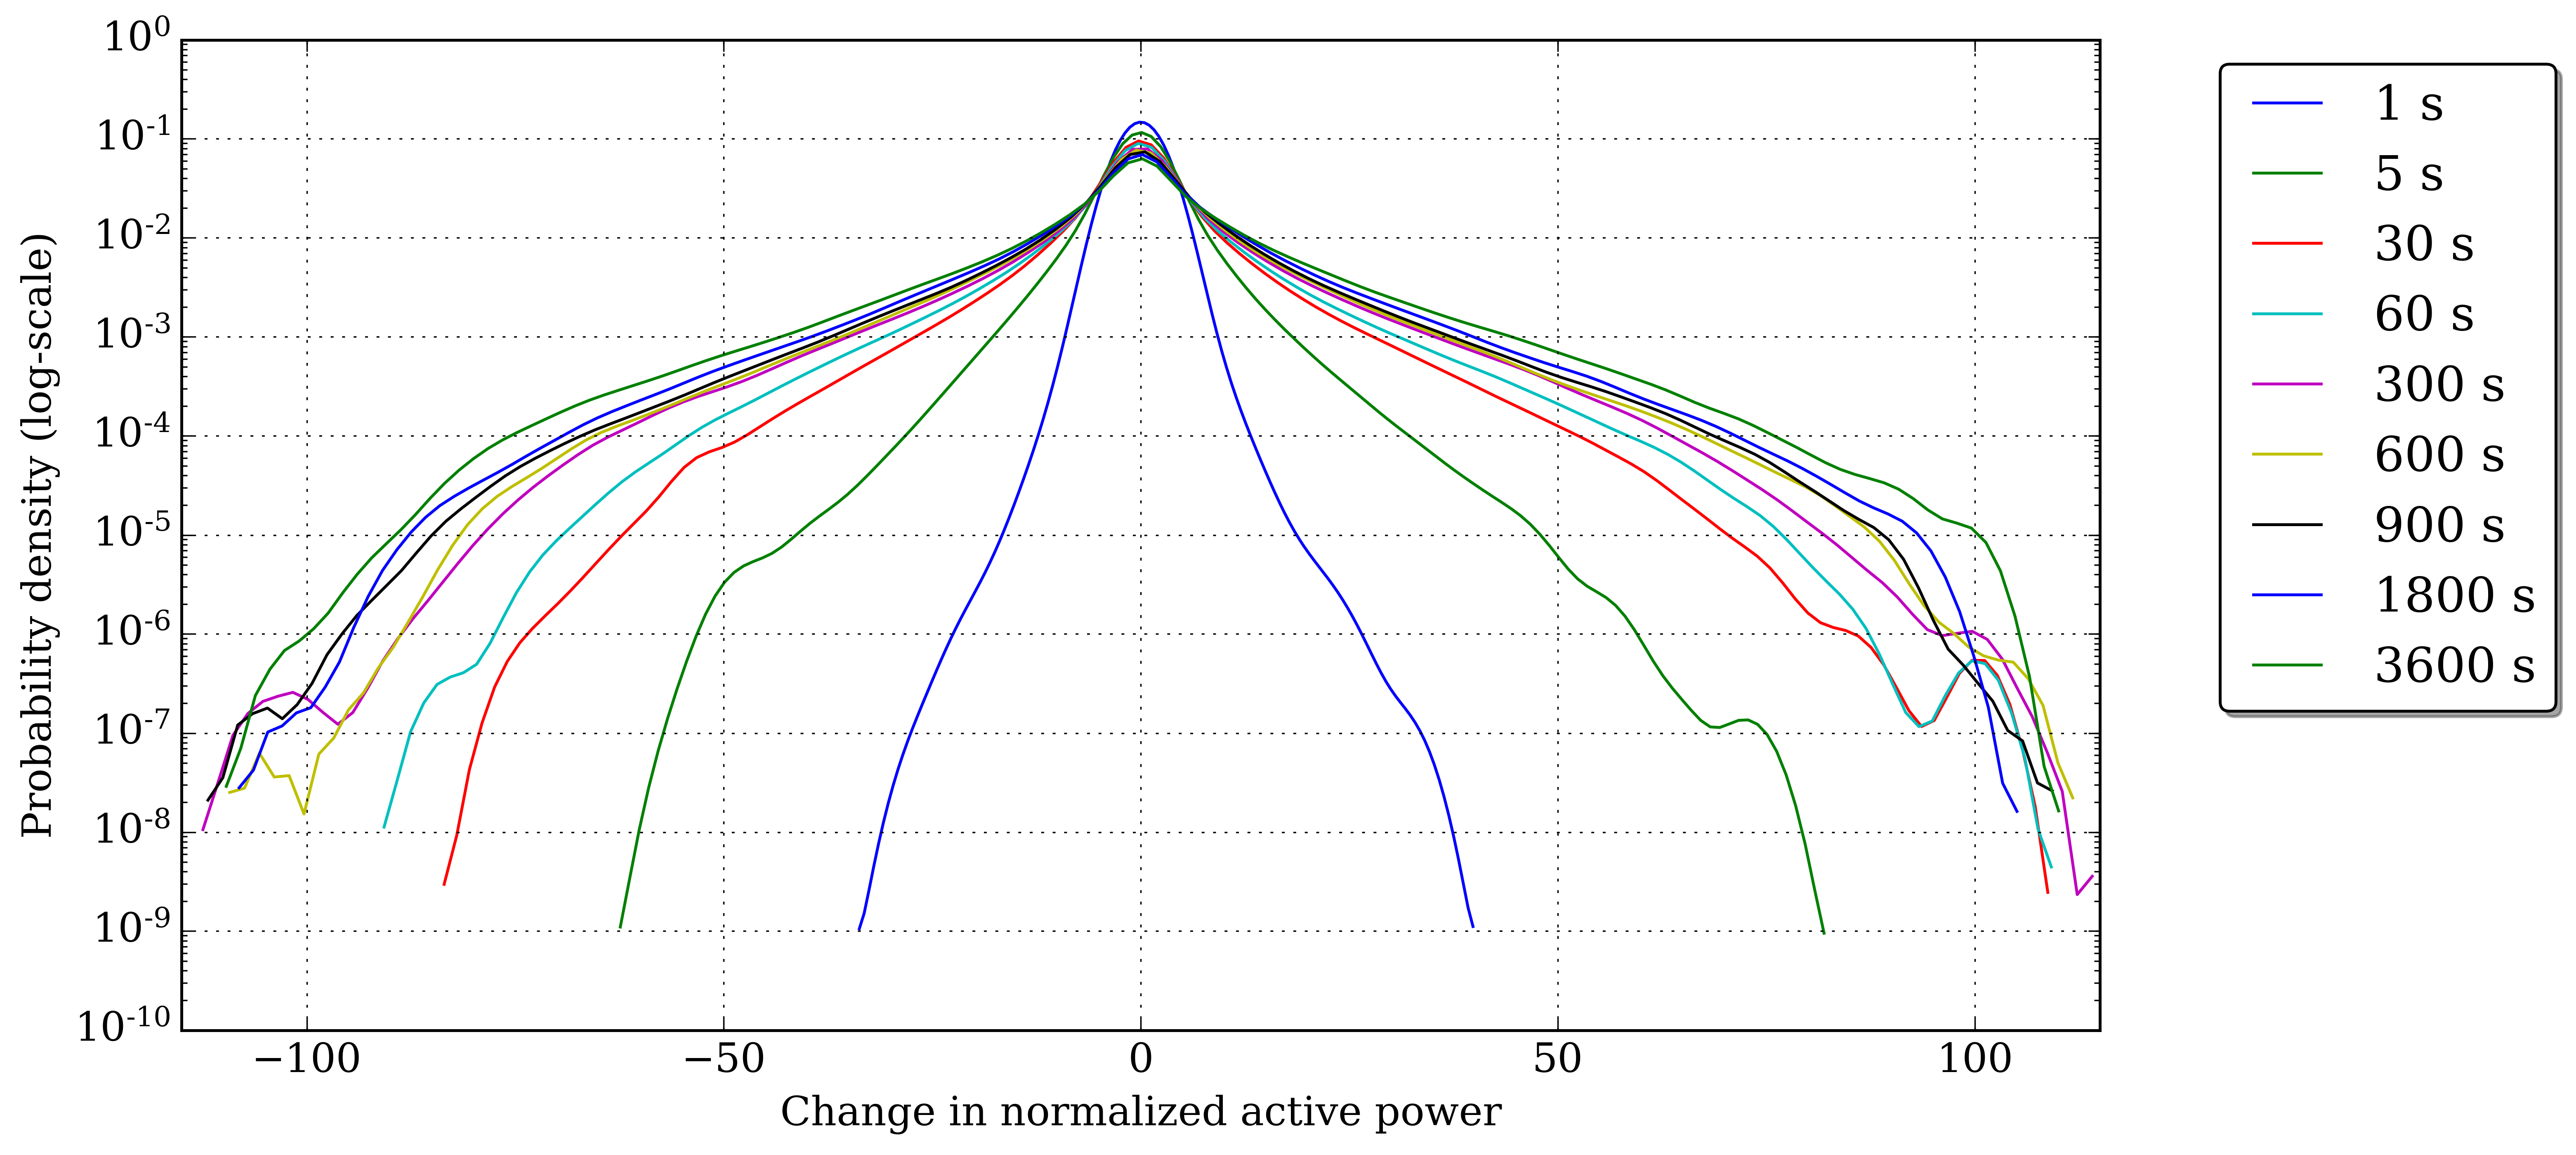
\includegraphics[width=1.0\textwidth]{graphics/intro/variability/norm_act_pow_error_dist.png}
    \caption{Distribution of changes in normalized active power over various time horizons from DTU's V52 research wind turbine}
    \label{fig:norm_act_pow_error_dist}
\end{figure}

This simplified investigation has considered a single wind turbine and not collective wind farm output or otherwise geographically distributed generation which will act to some degree as a smoothing filter. Having said that, the case study has demonstrated that minute-scale variability of wind power is not insignificant and attention should also be focused on this timescale alongside the more commonly focused periods (e.g. 10-minutes and 1-hour).

%--------------------------------------------------------------------------------
\clearpage
\subsection{Wind farm control}
\label{sec:intro_control}

Utility scale wind power installations consist of multi-turbine arrangements known as wind farms. The layout is normally characterized by rows of turbines which affect each other through complex aerodynamic interactions. The most notable being wake induced power losses (through a reduction in the extractable energy of the wind by upstream turbines) and fatigue loading (by increased turbulence originating from the air-blade interaction of upstream turbines).

Modern wind turbines are designed with control systems which act to optimize their performance from an individual perspective. However, all together this greedy approach does not always result in the best coordination of the wind farm as a whole. The field of wind farm control aims to collectively optimize the power and loads of the entire wind farm in a collaborative manner by orchestrating control over each turbine's set-points. The overall objectives being to either maximize total active power or provide power control by following a reference signal, and to minimize fatigue loads (\cite{knudsen_survey_2015}). The two main mechanisms for dynamic wind farm control are induction control and wake steering.

Axial induction control reduces the velocity deficit of the downstream wake leading to larger amounts of recoverable energy available to downstream turbines. A wind turbine's power coefficient at its maximum operating point is much less sensitive to changes in pitch angle than its thrust coefficient (\cite{annoni_analysis_2016}). Exploiting this relationship allows for small decreases in the upstream turbine's production to be more than made up for by increased production at the downstream turbines. This is accomplished by slightly pitching the rotor outwards (towards feathered position) and adjusting the generator torque which results in a decrease in the power and thrust coefficients and a reduction in the tip speed ratio. Normally this is performed by reducing the active power of the turbine (downrating), instead of manually interfacing with the turbine's pitch and torque set-points. \cite{gebraad_maximum_2015} establishes a 1.36\% improvement in annual energy production (AEP) using dynamic induction control simulations at the Princess Amalia Wind Farm in the Netherlands. Induction control using static set-point optimization has demonstrated far less promise, with no net increase in wind farm efficiency during wind tunnel testing (\cite{bartl_experimental_2016}).

Wake steering is the intentional misalignment of an upstream turbine's rotor in order to redirect (steer) the wake away from downstream turbines. During normal operation, the turbine will orient its rotor perpendicularly to the wind direction. Applying wake redirection causes the turbine's yaw motor to re-orient itself to an angle relative to the wind direction (Fig. \ref{fig:wake_steering}). This causes the wake to deflect away from downwind turbines, leading to a net increase in energy production for the overall wind farm. Positive yaw misalignment angles are normally used, as this results in a positive tilt angle which also directs the wake downwards. Simulations have indicated the potential for power gains using this approach while also avoiding significant load repercussions. The gains in AEP are on the order of 5\% through the reduction of wake losses (\cite{knudsen_survey_2015}, \cite{gebraad_maximization_2017}). The concept has been successfully demonstrated in a recent field trial (\cite{fleming_field_2017}) which confirms the simulation estimates.

\begin{figure}[htbp]
    \centering
        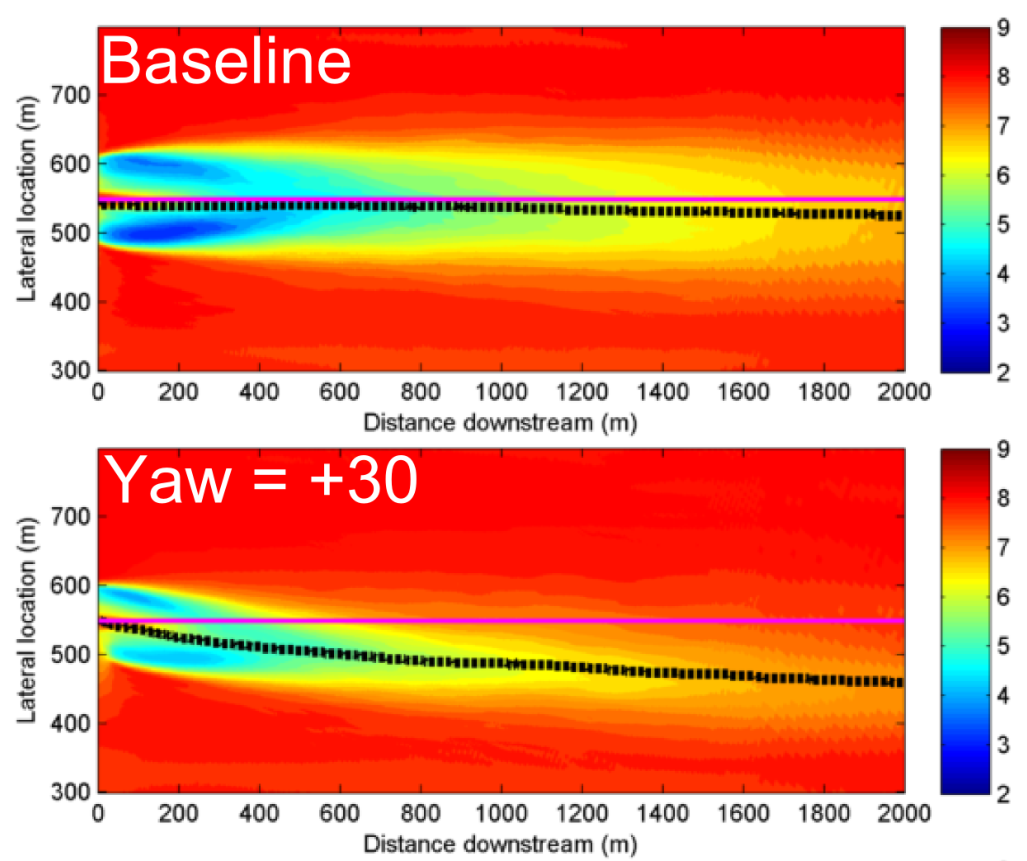
\includegraphics[width=0.5\textwidth]{graphics/intro/wake_steering.png}
    \caption{Comparison of the horizontal wake during normal operation (top panel) and under wake steering control (bottom panel, 30\degree \ yaw misalignment). The actual wake center-line is indicated in black, with the linear downstream reference in pink. Simulation using NREL's SOWFA toolbox in OpenFOAM. Reproduced from: \cite{fleming_wakesteering_2014}}
    \label{fig:wake_steering}
\end{figure}

Wind farm control algorithms require estimates of the incoming wind speed and direction. These inputs are used in a wind farm flow model together with a delay factor to account for the wind field advection between turbine rows. The forecasts are applicable on the minute scale for preemptive optimization by the wind farm controller and for the individual turbines to adjust their configurations accordingly. Induction control is sensitive to accurate wind speed inputs, while wake steering is sensitive to accurate wind direction inputs. Improved forecast performance on this timescale therefore also enhances the benefits of dynamic wind farm control.

The field of individual turbine control (i.e. feed-forward and model predictive control) is largely irrelevant in the context of this project, as the timescales are in the order of seconds ahead where direct advection (frozen turbulence) models perform sufficiently well. There may be a case for individual turbine yaw control on the minute scale, however this is seen as a low priority application with limited relative benefits over existing solutions.

%--------------------------------------------------------------------------------
\clearpage
\subsection{Forecasting for wind energy}
\label{sec:intro_forecasting}

The evolution of wind power together with advancements in computing and an improved understanding of atmospheric dynamics has established forecasting as a central element of operational research. An entire sub-industry is dedicated to developing and providing forecasting services to end users which include: wind farm owners and operators, power traders, asset managers, and transmission system operators (TSOs).

Wind prediction is conducted on a wide range of time scales, with lead times spanning from a few milliseconds up to one week or more. Prediction intervals can be described by a few broad categories, each with their own approaches and applications. Table \ref{tab:forecast_overview_table} outlines the common forecast horizons relevant to wind energy and typical methods applied within them. Broad overviews of the field are also presented in \cite{costa_review_2008}, \cite{giebel_state---art_2011} and \cite{soman_review_2010}.

\begin{table}
    \centering
    \caption{Overview of forecast intervals of interest for wind energy purposes}
    %\resizebox{\textwidth}{!}{%
\begin{tabular}{|l|l|l|l|l}
\large
\cline{1-4}
Designation & \textbf{Typical horizon} & \textbf{Example methods} & \textbf{Example applications} &  \\ \cline{1-4}
\textbf{Immediate} & \begin{tabular}[c]{@{}l@{}}Milliseconds\\ to seconds\end{tabular} & \begin{tabular}[c]{@{}l@{}}--- Persistence\\ --- Wind field measurements using nacelle lidars {[}1{]}\\     and/or upwind turbine SCADA {[}2{]}\end{tabular} & \begin{tabular}[c]{@{}l@{}}--- Wind turbine control {[}1{]}\\ --- Grid regulation {[}3{]}\\     (e.g. frequency, voltage support)\end{tabular} &  \\ \cline{1-4}
\textbf{\begin{tabular}[c]{@{}l@{}}Very short-term \\ (minute scale)\end{tabular}} & \begin{tabular}[c]{@{}l@{}}1-minute\\ to 1-hour\end{tabular} & \begin{tabular}[c]{@{}l@{}}--- Persistence {[}4{]}\\ --- Statistical time series models {[}5{]}\\ --- Markov (regime switching) models {[}6{]}\\ --- Machine learning and artificial neural networks (ANN) {[}7,8{]}\end{tabular} & \begin{tabular}[c]{@{}l@{}}--- Wind farm control\\ --- Ancillary services \\     (e.g. reserve power) {[}2,9{]}\\ --- Intrahour energy market trading {[}10{]}\\ --- Storage management\\     (e.g. battery storage control)\end{tabular} &  \\ \cline{1-4}
\textbf{Short-term} & 1 to 72 hours & \begin{tabular}[c]{@{}l@{}}--- Statistical time series models {[}11,12{]}\\ --- Numerical weather prediction (e.g. WRF) {[}13{]}\\ --- Analogue ensemble prediction {[}13,14{]}\\ --- Kalman filter {[}11,15{]}\end{tabular} & \begin{tabular}[c]{@{}l@{}}--- Intraday and day-ahead energy market trading {[}10{]}\\ --- Ancillary services\\ --- Storage management\\     (e.g. battery, hydrogen and pumped storage control) {[}16{]}\\ --- Economic dispatch and generator planning\\ --- Operator portfolio management\end{tabular} &  \\ \cline{1-4}
\textbf{Long-term} & \begin{tabular}[c]{@{}l@{}}72 hours \\ to 10 days or more\end{tabular} & \begin{tabular}[c]{@{}l@{}}--- Same as short term\\ --- Climatology\end{tabular} & \begin{tabular}[c]{@{}l@{}}--- Reserve requirement decisions\\ --- Unit commitment decisions\\ --- Maintenance scheduling\end{tabular} &  \\ \cline{1-4}
\end{tabular}
}
    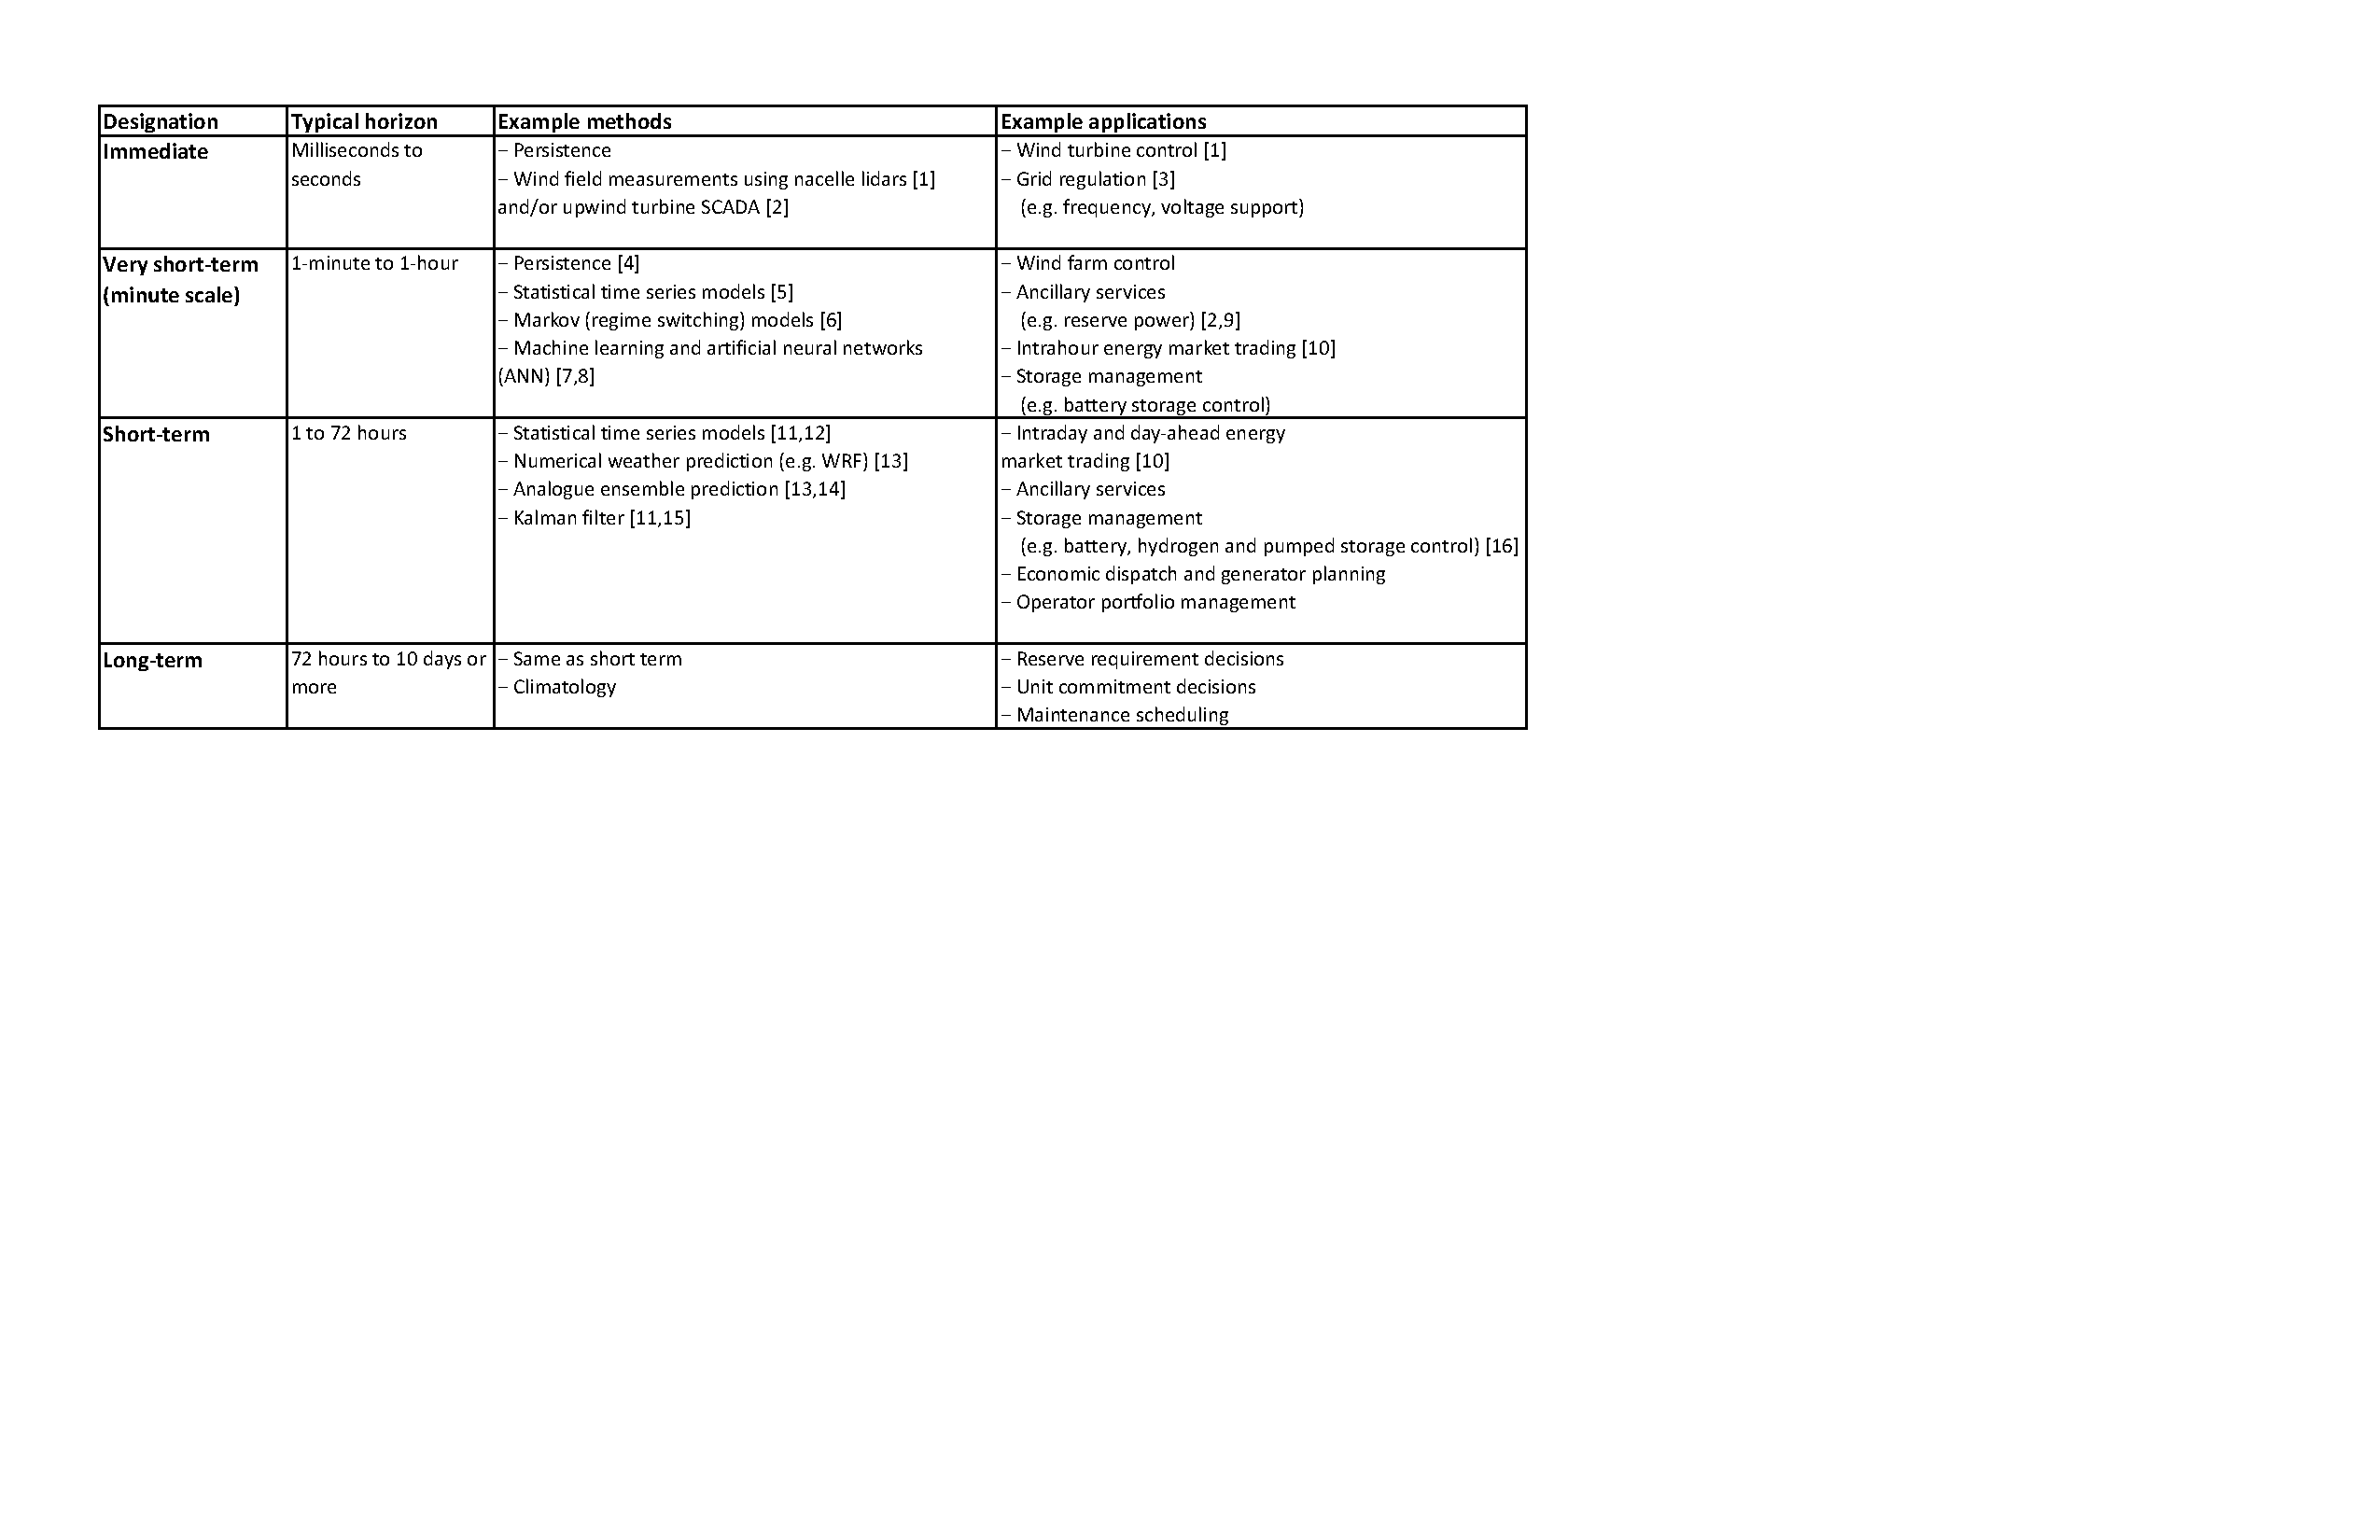
\includegraphics[width=1.0\textwidth]{tables/forecast_overview_table.pdf}
    \resizebox{\textwidth}{!}{%
\begin{tabular}{|c|}
\hline
\textbf{References} \\ \hline
\begin{tabular}[c]{@{}c@{}}
{[}1{]} \cite{schlipf_nonlinear_2012}, 
{[}2{]} \cite{gocmen_possible_2016}, 
{[}3{]} \cite{hansen_provision_2016}, 
{[}4{]} \cite{hodge_wind_2011}, 
{[}5{]} \cite{pinson_very_2012}, 
{[}6{]} \cite{trombe_general_2012}, \\ 
{[}7{]} \cite{potter_very_2006}, 
{[}8{]} \cite{niu_multi-step-ahead_2018}, 
{[}9{]} \cite{mackenzie_short-term_2017}, 
{[}10{]} \cite{bathurst_trading_2002}, 
{[}11{]} \cite{liu_comparison_2012}, \\ 
{[}12{]} \cite{torres_forecast_2005}, 
{[}13{]} \cite{mahoney_wind_2012}, 
{[}14{]} \cite{delle_monache_probabilistic_2013}, 
{[}15{]} \cite{bossanyi_short-term_1985}, 
{[}16{]} \cite{castronuovo_integrated_2013}
\end{tabular} \\ \hline
\end{tabular}
}
    \label{tab:forecast_overview_table}
\end{table}

Forecasting techniques can be categorized into two fundamental classes- process driven physical models and data driven statistical approaches. Here general introductions are given for both. An extensive review is provided in Section \ref{sec:IEA_paper}.

Physical approaches such as numerical weather prediction (NWP) are based on well established physical and mathematical laws. Parameterizations of the atmosphere, where coarse input data (global or synoptic scale) is combined with mathematical modelling of atmospheric properties such as air, soil and sea temperature, pressure, land cover and surface obstacles to provide a local site forecast at varying temporal and spatial resolutions. Optionally, through data assimilation the model states can be iteratively adjusted using real-time observations to adapt the simulation and correct for biases. These systems generally run on large supercomputers and require significant time and computational power to generate their forecasts. Further, they have not sufficiently demonstrated their ability to predict local microscale events that are of greatest relevance for real-time wind farm control. Therefore they are not considered appropriate in the context of minute-scale wind forecasting as they are ill-suited to be used operationally with today's computing technology.

Statistical approaches use empirical methods to model relationships between historical observations. The models are then used with real-time inputs to extrapolate future outcomes. Meteorological data is normally given as a time-series, where samples are highly correlated, non-independent and naturally ordered in time. The high temporal autocorrelation of wind measurements lends itself well to the simplest statistical approach called persistence. Persistence simply forecasts the future value of the series to be the same as the most recent observation, or a moving average of it. This method is widely used on horizons from the immediate to short-range, and is a common benchmark for evaluating more complex techniques. Autoregressive (AR) models are also appropriate, and are widely employed, often in conjunction with moving average (MA) models. In cases where the target signal is non-stationary, a number of transformation steps can be taken to impart stationarity (e.g. differencing, trend removal, seasonal and cyclical adjustments). Formulations which have demonstrated particularly adept skill are autoregressive integrated moving average (ARIMA) models. Further details on ARIMA modelling are given in Section \ref{sec:lascar_paper}. The flexibility of statistical approaches empower their suitability for minute-scale forecasting applications. This thesis work therefore exists within this research topic.

\begin{comment}
Evaluating forecasts?
\end{comment}

%--------------------------------------------------------------------------------
\clearpage
\subsection{Power system and electricity markets}
\label{sec:intro_power_markets}

The vast majority of wind power installations are grid connected and offer the sale of their production through either long term power purchase agreements (PPA) or via wholesale electricity spot markets.

The modern electrical grid is a network of providers and consumers of electrical energy, interconnected via transmission and distribution lines used to transport supply from generation facilities to homes and businesses. Electrical appliances are designed to operate within a narrow range of the design frequency and voltage of the local AC power grid. Deviations can result in malfunctions or damage, or even in cascading failures as devices such as pumps, fans, motors, and power electronics drift from their intended output or stop functioning completely. For this reason, the supply and demand of electricity must be kept in constant balance. Variability occurring on both sides of the equation (load and generation) drives a need for accurate forecasts, which are used in system planning and generator dispatch. Deviations from the equilibrium between generation and consumption requires real-time adjustments, directed by the balancing authority (BA) through the activation of a suite of ancillary services to ensure stable frequency and voltage levels. Traditionally, wind power plants have not participated in these ancillary services. Grid codes are beginning to allow such involvement, for example tertiary regulation and deviation management in Spain (\cite{ignacio_de_la_fuente_ancillary_2016}), and minute-scale reserves in Germany through the intentional down-regulation of wind farms (\cite{regelleistung_leitfaden_2016}).

Energy markets attempt to provide the optimum allocation of resources through the minimization of pricing while fulfilling balance constraints. This is enacted through an auction style clearing process, where utilities place bids to cover the forecasted demand of their customers, and generators place bids to offer their production into the market. The market price is then set at the intersection of the supply and demand offers, which is calculated for each region (i.e. zone or node). The market is subdivided geographically to account for constraints in transmission capacity, with import/export links considered. Once offers are accepted, participants are balance responsible (BRP) for delivering their scheduled quota within the given trading block. If any deviations occur, they may incur financial penalties depending on the effect of their imbalance (i.e. helping or hurting the system). It is common for market operators (e.g. in NordPool's two-price system) to discourage gaming tactics by preventing revenues from exceeding initial market payouts through exploiting up- and down-regulation price movements.

Market design is highly dependent on location, but exchanges often operate day-ahead and intraday markets with trading segments in one hour blocks, and with long lead times between bid placement and delivery. These lengthy intervals create issues for variable renewables such as wind. Market operators in regions with high penetrations of renewables are moving to shorten these horizons, in certain cases to continuous intraday markets with 5, 15, and 30 minute contracts (\cite{epex_spot_se_continuous_2019}, \cite{aemc_five_2017}) where minute-scale wind forecasts become relevant and necessary for traders.



\begin{comment}
Errors in power forecast do not necessarily reflect impact. Overestimation and underproduction != underprediction and overproduction due to structure of balancing market.
The need for spinning reserves. Frequency control/response mode. Droop speed control. Spinning reserve is extremely expensive for utilities. 
https://en.wikipedia.org/wiki/Dynamic_demand_(electric_power)#The_need_for_spinning_reserve
Cost of imbalance not only money but also CO2
\end{comment}

%--------------------------------------------------------------------------------
%\clearpage
%\subsubsection{Case study of wind power operation in a 5-minute energy market}
%\label{sec:intro_aus_power_study}

%Placeholder for Australian energy market case study


%--------------------------------------------------------------------------------
%--------------------------------------------------------------------------------
\clearpage
\section{Remote sensing of winds}
\label{intro_remote_sensing}

For centuries wind measurements in the atmospheric boundary layer (ABL) have been performed using a variety of in situ techniques, where instruments including cup anemometers and wind vanes are mounted on towers to measure the local flow at the sensor's position. These methods are often employed within wind energy for resource assessment and site suitability studies, and for turbine power performance testing.

The increasing scale of modern wind turbines (e.g. the 9.5 MW Vestas V164 and GE's upcoming 12 MW Haliade-X) has resulted in rotor tip heights approaching 300 m, which represents both a financial and technical challenge when relying on mast based measurements, particularly in offshore environments.

Remote sensing (RS) is a measurement process in which observations are made at a distance (i.e. without being physically present at the target position). This provides a number of advantages in the flexibility and cost of running a measurement campaign, and in enabling new ways to measure.

For performing wind measurements, active RS devices are designed to utilize the Doppler effect to obtain velocity information. This is done by emitting an electromagnetic or sound wave of a known frequency which backscatters off of objects within the measurement volume and is acquired again by the receiver (e.g. telescope, parabolic dish, microphone). The returned signal is analyzed (either directly or using coherent detection methods) and the radial velocity is determined through its proportionality to the frequency shift using spectral estimation. The obtained radial velocity represents the wind velocity projected along the beam's path (line of sight, LOS). In the case of atmospheric measurements, the target objects are aerosols- particles such as dust, water vapor, and particulate matter (pollutants) which are suspended in the air and are assumed to be moving together with the wind.

% (Eq. \ref{eq:doppler_shift})
%\begin{equation}
%    \centering
%        \Delta f=2 \frac{u_{r}}{c}
%    \label{eq:doppler_shift}
%\end{equation}
%\noindent
%where $\Delta f$ is the Doppler shift, $u_r$ is the radial wind speed, and $c$ is the speed of light.

Relevant RS devices represent a wide class of technologies such as Doppler radar, Doppler sodar, and Doppler lidar which can be ground based, nacelle mounted, on fixed or floating platforms, or on space-borne satellites. Each tool has its own advantages and disadvantages. Operational pulse Doppler radar systems typically have large antennas and high powered transmitters which enable them to measure at far distances (e.g. up to 300 km for S-band Nexrad systems in the US observation network). However, they require precipitation for reflectivity and the range resolution is insufficient for detecting small scale motion, especially at further distances. Ka-band Doppler radars have been developed which are more compact and are able to measure in clean air up to 30 km (\cite{hirth_measuring_2012}). These devices show potential for providing real-time microscale wind field measurements, however initial reports on data availability have been disappointing. In this thesis we will focus solely on Doppler wind lidar systems due to their portable size, commercial availability, well established performance, and capability of measuring in diverse atmospheric conditions. Compact pulsed lidar variants have a typical maximum range on the order of 10 km, which corresponds to advection occuring up to 30-minutes ahead, depending on wind speed.

%Space born systems including synthetic aperture radars and the recently launched ALADIN lidar profiler on ESA's ADM-Aeolus satellite offer global coverage at the expense of spatial and temporal resolution.


%--------------------------------------------------------------------------------
%\subsection{Principles}
%\label{sec:intro_rs_principles}
%--------------------------------------------------------------------------------
\clearpage
%\subsection{Pulsed coherent Doppler lidar}
\subsection{Doppler wind lidars}
\label{sec:intro_lidar}

Doppler wind lidars are active remote sensing instruments which use laser light in the near-infrared band as their medium. The laser source is in most cases a 1.5 $\mu$\\m all-fiber laser, which corresponds to the spectral absorption line of atmospheric water vapor and carbon dioxide while also satisfying eye safety requirements (\cite{cariou_laser_2006}). An added benefit is that this application overlaps with fiber optic components used in the telecommunications industry. This has resulted in affordable and widely available hardware options for manufacturing the lidar's optical systems.

Doppler wind lidars are built commercially in a variety of configurations depending on the mounting location and measurement setup. The simplest systems have fixed telescopes which stare or switch between predetermined beam positions and are commonly used in nacelle lidars. Units with a rotating platform and offset mirror or prism perform repeating conical scans along a fixed path and are commonly used in certain lidar wind profilers. Scanning lidars are equipped with a dual-axis scanner head which allows the beam to be pointed arbitrarily in space, with little restrictions on the path, timing, and geometric complexity of the scanning trajectory (subject to the kinematic constraints imposed by the mechanical design). Fig. \ref{fig:lidars} presents a look at some of the most common commercially available lidar systems.

\begin{figure}[htbp]
    \centering
        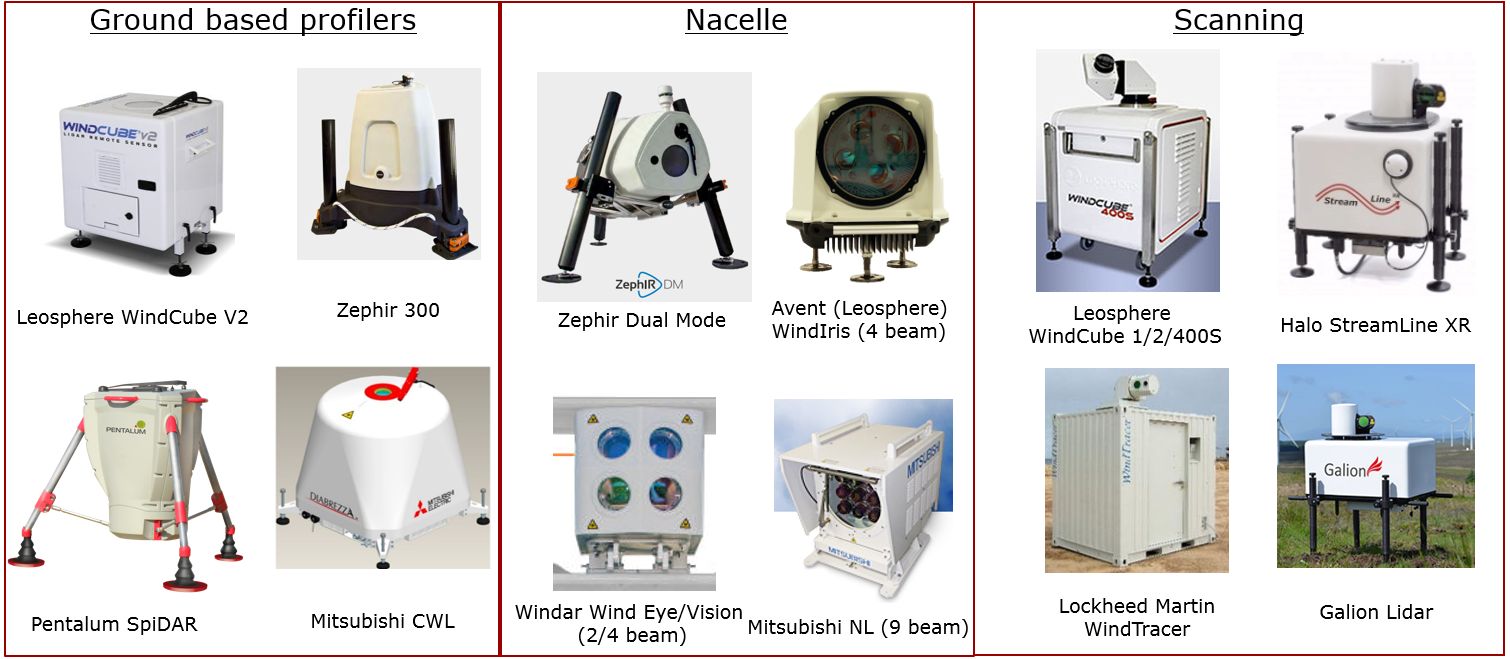
\includegraphics[width=1.0\textwidth]{graphics/intro/lidars.png}
    \caption{Selection of commercially available lidar systems, grouped by main function. Images sourced from the manufacturer's respective product brochures}
    \label{fig:lidars}
\end{figure}

Two main diverging classes of lidar technology exists- pulsed and continuous-wave (CW) systems, which differ greatly in their spatial and temporal resolutions. CW lidars emit a continuous focused beam, which must be re-focused for different measurement ranges. The spatial resolution of a CW lidar is directed by the aperture of the telescope, which results in an increase in the probe length as a function of the square of the range. This implies that CW lidar technology is only suitable for close ranges, up to a few hundred meters away. In contrast, pulsed lidars emit a collimated beam using a series of short pulses on the order of nanoseconds. This allows all distances along a pulsed lidar's laser path to be measured at once, using time-of-flight calculations to discern the appropriate distances into range gates (RG) without any change in spatial resolution with distance (i.e. the probe length is fixed, but the intensity of the returned signal is reduced by the square of the range). Coherent pulsed Doppler lidars equipped with high powered optical amplifiers are capable of measuring up to 30 km, although compact units are usually limited to between 5-12 km. For these reasons, pulsed lidar variants show the most promise in terms of suitability towards applications which cover large spatial scales, including minute-scale forecasting.

\begin{comment}
Pulsed Doppler lidar measurement chain
Practicalities
\end{comment}

%--------------------------------------------------------------------------------
\clearpage
\subsection{Measurement techniques}
\label{sec:intro_meas_tech}

As introduced in Section \ref{sec:intro_lidar}, application specific lidar systems normally follow preset scanning strategies, while scanning lidars allow for more complex measurement techniques. A brief synopsis of available measurement configurations for a coherent pulsed scanning Doppler lidar is given in the following: 

\begin{itemize}
\item LOS (staring mode) --- The beam position remains fixed and measurements are acquired continuously at the target point.

\item DBS (Doppler beam swing) --- A technique used to measure vertical wind profiles by measuring at typically four orthogonal positions around a cone and optionally including a fifth central beam to directly measure the vertical wind component. The conical radial speed observations exhibit a cosine function. Fitting techniques are then used to produce estimates of the wind vector components by assuming the wind is frozen and horizontally homogeneous between the discrete sampling points.

\item VAD (velocity azimuth display) --- Also used primarily for vertical wind profiling, but in certain cases is rotated for horizontal use. The elevation angle is held constant while sweeping across the full range of azimuths. This performs a full conical scan which can be fit similarly to the DBS technique.

\item PPI (plan position indicator) --- Closely related to the VAD method, PPI scans use fixed, low (or flat) elevation angles and sweep across a full or partial range of azimuths. This results in conical arc slices over a large horizontal distance. The radial speed signals similarly follow a cosine function, with the peak and trough corresponding to the azimuth position aligned into and away from the wind direction. When the beam is perpendicular to the wind, the observed radial speed is zero. PPI scans produce cross-sections of the horizontal wind structure and are processed using retrieval or fitting methods by assuming horizontal homogeneity and by not taking vertical effects into account.

\item RHI (range height indicator) --- The counterpart to PPI scanning, RHI scans vary the elevation axis while keeping the azimuth fixed. This produces cross-sections of the vertical wind structure along an arc.

\item User defined --- Complex trajectories which are custom tailored for the particular application are also possible. An example of this is the ridge transect scan used in the Perdig\~ao field campaign which follows the site's topography along a fixed height (\cite{robert_menke_perdigao_2017}).

\item Dual and triple Doppler --- Beams from multiple separated lidars can be intersected in space (and ideally time) to measure either two or all three of the wind velocity components with any of the above-mentioned scan patterns. The independent measurements are then combined together when performing the wind field reconstruction. Dual Doppler approaches have shown to slightly improve wind retrieval results in simple terrain compared to single Doppler techniques (\cite{simon_comparison_2016}, \cite{floors_report_2016}), while forgoing the assumption of horizontal homogeneity. However, this advantage is offset by the increased cost of the additional systems and reliance on data availability with all systems.

\item Dynamic --- The previously described scan types are normally configured in advance and set to repeat continuously, or to cycle through a predetermined set of scans along a schedule. Dynamic scanning adapts the lidar's trajectory to real-time inputs, chiefly those derived from the measurements themselves such as wind speed and direction. An example includes \cite{wildmann_wind_2018} which adjusts parameters of the scan to follow the downstream turbine wake through changes in the wind direction.

\end{itemize}

These scanning strategies can be configured and combined to suit the measurement objective and take site-specific particularities into account. This allows for ultimate flexibility in the placement of devices, measurement range and spatial resolution, sampling rate of the data, and spatial 


\begin{comment}
Filtering techniques
\end{comment}

%--------------------------------------------------------------------------------
%\clearpage
%\subsection{Processing, filtering, and interpreting data}
%\label{sec:intro_rs_data}

%TODO:
%\begin{itemize}
%\color{red}
%    \item Data formats
%    \item Filtering techniques
%    \item Interpreting measurements
%\end{itemize}

\clearpage